\chapter{Implementación hardware}

Para implementar el algoritmo en hardware dividimos en módulos el algoritmo de filtrado, el algoritmo
de deteccion de picos y el algoritmo de deteccion de arritmias, estos los unificamos en un super módulo 
y probamos la simulacion con un testbench.

Como los valores de las señales estan en punto flotante para operar con ellos es necesario utilizar módulos
hardware que permitan hacer dichas operaciones, en este proyecto utilizaremos módulos de resta, division y 
comparacion de numeros en punto flotante.

\section{Módulo de filtrado}

Este módulo utiliza una ROM con los coeficientes, una RAM con las muestras y un módulo de multiplicacion
de numeros en punto flotante.

Este módulo se compone de una maquina de estados que va multiplicando cada elemento de la RAM muestras 
con los elementos de la ROM coeficientes con el módulo de multiplicacion de punto flotante.

\subsection{Señales de entrada y salida}

Las señales de entrada son:

\begin{itemize}
\item clk y reset
\item input\_signal\_data: señal que recibe las muestras de la señal original 
\item input\_valid e input\_ready: son flags que sirven para sincronizar el módulo con la llegada de muestras. 
\end{itemize}

Las señales de salida son:

\begin{itemize}
    \item output\_filter\_data: saca los valores de la señal filtrada
    \item output\_filter\_index: saca los indices de cada valor de la señal filtrada
    \item output\_valid y output\_ready: se encargan de sincronizar el módulo del filtrado 
    con el módulo de deteccion de picos
\end{itemize}



\lstset{language=VHDL, breaklines=true, basicstyle=\footnotesize}
\begin{lstlisting}[frame=single]
    entity filter is
    port (
        -- Seniales de reloj y de reset
        clk                 : in  std_logic;
        reset               : in  std_logic; 
        
        -- bus AXI Stream de entrada
        input_signal_data   : in  std_logic_vector(31 downto 0);
        input_valid         : in  std_logic;
        input_ready         : out std_logic;
        
        -- bus AXI Stream de salida
        output_filter_data  : out std_logic_vector(31 downto 0);
        output_filter_index : out std_logic_vector(31 downto 0);
        output_valid        : out std_logic;
        output_ready        : in  std_logic   
   );
end filter;
\end{lstlisting}

\begin{figure}[h!]
    \centering
    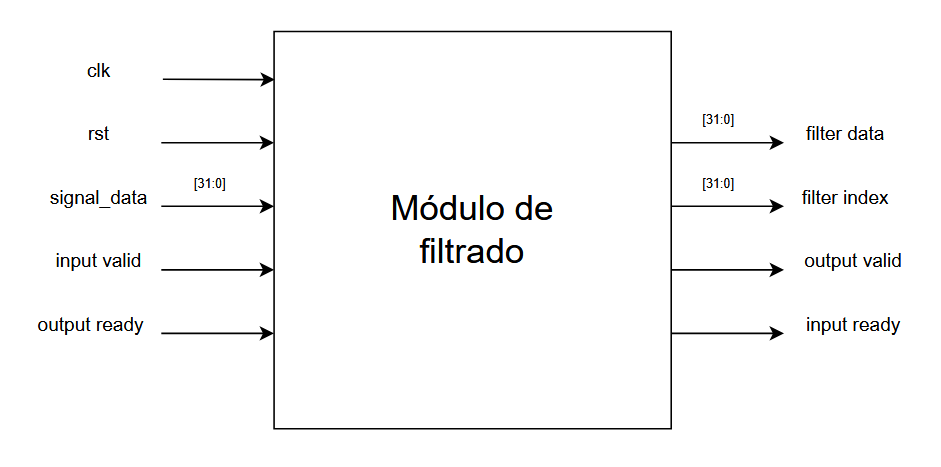
\includegraphics[width=0.8\textwidth]{./Images/img_implementacion_hw/modfiltrado.png}
    \caption{Entradas y salidas del módulo de filtrado}
    \label{fig:modfiltrado}
\end{figure} 

\subsection{Maquina de estados}

\begin{figure}[h!]
    \centering
    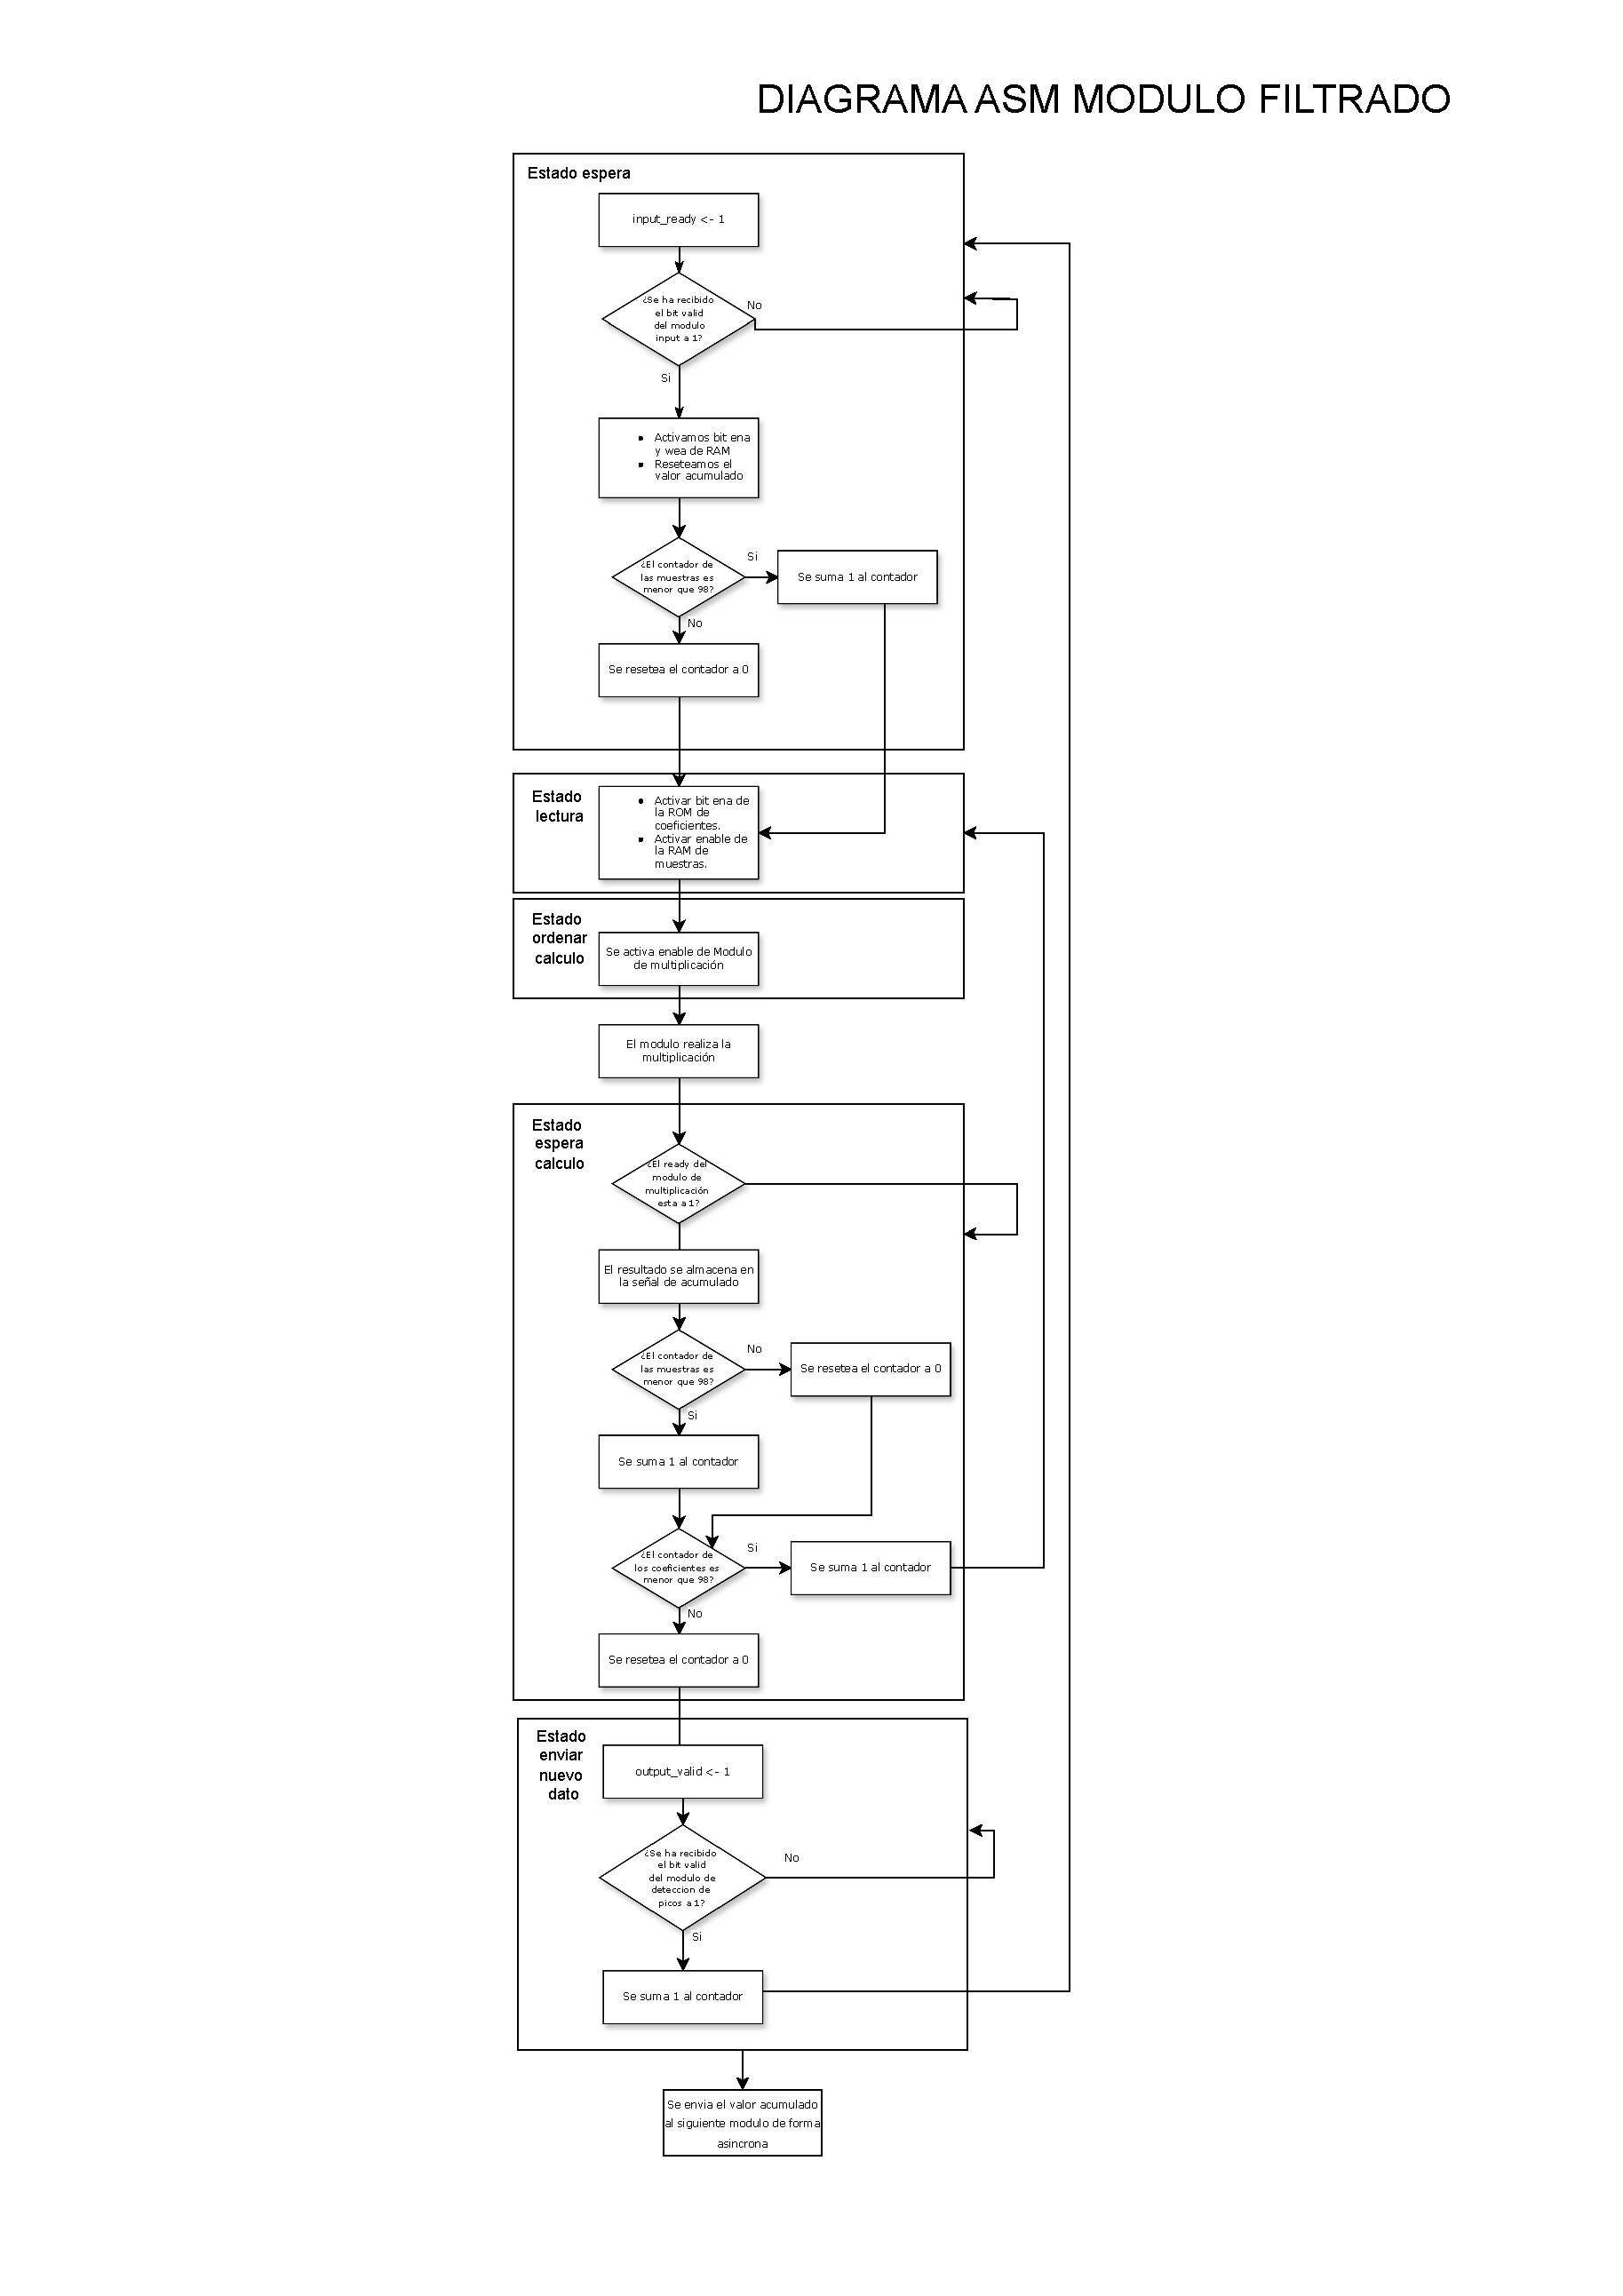
\includegraphics[width=0.99\textwidth]{./Images/img_implementacion_hw/Diagramaasmfiltrado.pdf}
    \caption{Diagrama asm de Módulo de filtrado de señal}
    \label{fig:Diagramaasmfiltrado}
\end{figure} 

El envio de datos al output se realiza de forma asincrona
\lstset{language=VHDL, breaklines=true, basicstyle=\footnotesize}
\begin{lstlisting}[frame=single]
    output_filter_data <= acumulado;
    output_filter_index <= cont_indice;
\end{lstlisting}

\begin{itemize}
    \item Estado de espera: En el estado de espera se activa la señal de ready y se espera a que se envie un valor de la
    señal sin filtrar, se borra el valor de la solucion de la multiplicacion anterior en caso de haberla, se activan las
    señales de escritura de la RAM y se establece el indice donde se va a escribir la muestra.
    \item Estado lectura: Se activa la lectura de los coeficientes y de las muestras.
    \item Estado para ordenar el cálculo: en este estado se activa el flag del módulo de multiplicacion.
    \item Estado de espera del calculo: se espera a que termine el módulo de multiplicacion esperando la señal de ready\_muladd
    y se almacena el resultado, tambien se actualiza el contador de los coeficientes, de las muestras y dependiendo de si el 
    indice de coeficientes es menor que 98 se va al estado de lectura o el estado de enviar un nuevo dato al siguiente módulo.
    \item Estado de envio de nuevo dato: este estado sincroniza el siguientemódulo, activa el bit de valid a 1 y espera el bit
    de ready del siguiente módulo para poder enviar el dato.
\end{itemize}

\subsection{Módulos utilizados}
Se utilizo una ROM para almacenar los coeficientes y poder leerlos

\lstset{language=VHDL, breaklines=true, basicstyle=\footnotesize}
\begin{lstlisting}[frame=single]
    -- ROM que contiene los coeficientes 
    ROM_coeficientes_i : entity work.ROM_coeficientes port map (
        clka      => clk,
        ena       => ROM_coeficientes_ena,
        addra     => ROM_coeficientes_addra,
        douta     => ROM_coeficientes_douta
    );
    
    ROM_coeficientes_addra <= cont_coeficientes;
\end{lstlisting}

Se usa una RAM para poder leer y escribir en las muestras de la señal original.

\lstset{language=VHDL, breaklines=true, basicstyle=\footnotesize}
\begin{lstlisting}[frame=single]
    -- ROM que contiene las muestras 
    RAM_muestras_i : entity work.RAM_muestras port map (
        clka      => clk,
        ena       => RAM_muestras_ena,
        wea       => RAM_muestras_wea,
        addra     => RAM_muestras_addra,
        dina      => RAM_muestras_dina,
        douta     => RAM_muestras_douta
    );    
    
    RAM_muestras_addra <= cont_muestras;
    RAM_muestras_dina <= input_signal_data;
\end{lstlisting}

Se usa un módulo de multiplicacion para poder multiplicar los valores de las muestras con los valores de los coeficientes.

\lstset{language=VHDL, breaklines=true, basicstyle=\footnotesize}
\begin{lstlisting}[frame=single] 
    -- Multiplicacion y suma 
    mul_add_i : entity work.muladdpf port map (
        aclk                    => clk,
        s_axis_a_tvalid         => enable_muladd,
        s_axis_a_tdata          => RAM_muestras_douta,
        s_axis_b_tvalid         => enable_muladd,
        s_axis_b_tdata          => ROM_coeficientes_douta,
        s_axis_c_tvalid         => enable_muladd,
        s_axis_c_tdata          => acumulado,                
        m_axis_result_tvalid    => ready_muladd,
        m_axis_result_tdata     => result_muladd
    );
\end{lstlisting}

\section{Módulo de deteccion de picos}

Este módulo se encarga de detectar los picos de la señal filtrada. 
\subsection{Señales de entrada y salida}

    \begin{figure}[h!]
        \centering
        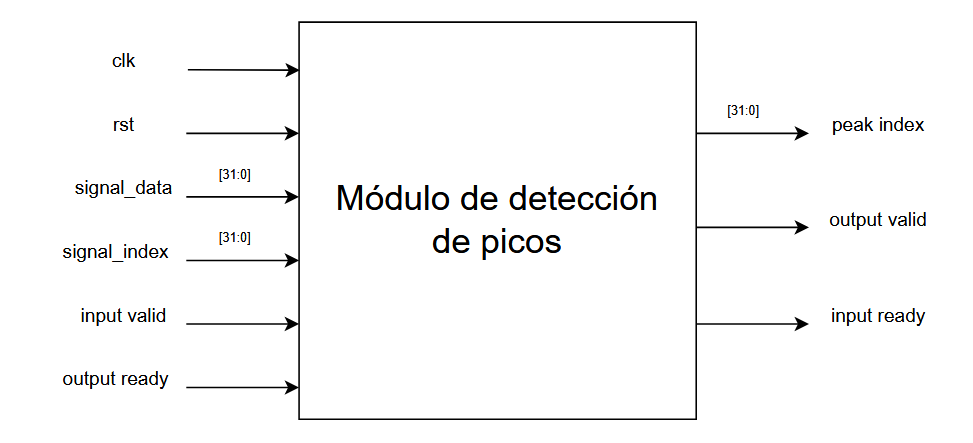
\includegraphics[width=0.6\textwidth]{./Images/img_implementacion_hw/moddeteccionpicos.png}
        \caption{Entradas y salidas del módulo de deteccion de picos}
        \label{fig:moddeteccionpicos}
    \end{figure} 
    
    \begin{itemize}
    \item clk y reset
    \item input\_signal\_data: señal que recibe las muestras de la señal filtrada 
    \item input\_signal\_index: señal que recibe lso indices de las muestras de la señal filtrada 
    \item input\_valid e input\_ready: son flags que sirven para sincronizar el módulo con la llegada de muestras. 
    \end{itemize}
    
    Las señales de salida son:
    
    \begin{itemize}
        \item output\_peak\_index: saca los indices de los picos detectados
        \item output\_valid y output\_ready: Se encargan de sincronizar el módulo de deteccion de picos 
        con el módulo de deteccion de arritmias.
    \end{itemize}

        
\lstset{language=VHDL, breaklines=true, basicstyle=\footnotesize}
\begin{lstlisting}[frame=single] 
port (
    -- Seniales de reloj y de reset
    clk                 : in  std_logic;
    reset               : in  std_logic; 
    
    -- bus AXI Stream de entrada
    input_signal_data   : in  std_logic_vector(31 downto 0);
    input_signal_index  : in  std_logic_vector(31 downto 0); -- vamos a dejarlo en 32 (aunque no sean necesarios tantos bits) para sean todos los buses iguales
    input_valid         : in  std_logic;
    input_ready         : out std_logic;
    
    -- bus AXI Stream de salida
    output_peak_index   : out std_logic_vector(31 downto 0); -- vamos a dejarlo en 32 (aunque no sean necesarios tantos bits) para sean todos los buses iguales
    output_valid        : out std_logic;
    output_ready        : in  std_logic   
);
\end{lstlisting}
\subsection{Maquina de estados}


\begin{itemize}
    \item Estado de espera: En el estado de espera se activa la señal de ready y se espera a que se envie un valor de la
    señal sin filtrar, se borra el valor de la solucion de la multiplicacion anterior en caso de haberla, se activan las
    señales de escritura de la RAM y se establece el indice donde se va a escribir la muestra.
    \item Estado de comprobar indice: si no hay pico, o lo que es lo mismo que la señal de last\_peak este a 0 este se asigna
     a la señal y ademas se registra el indice, despues pasa al estado de actualizar el cutoff activando por tanto la señal de 
     division para que empiecen los módulos de division y resta de valores en punto flotante a calcular el valor. Si por otro
     lado si que hay pico, se ordena hacer la comparacion signal\_data > last\_peak pasando las señales correspondientes al módulo de comparacion en 
     punto flotante. Ademas se anticipa y se hace la comparacion last\_peak > cutoff para en dado caso de que no se cumpla la 
     condicion anterior ya esta la comparacion hecha y se pude pasar directamente al estado siguiente. Tambien activamos las señales
     del módulo de comparacion correspondiente. El siguiente estado es el estado de espera a la condicion en la que la señal es mayor 
     que el pico maximo.
    \item Estado de actualizar cutoff: este estado espera a la señal ready del módulo de la resta ya que es la ultima operacion que se realiza para 
    calcular el cutoff. Primero se ejecuta el módulo de la division para calcular cutoff/192 y luego la resta cutoff - cutoff/192. cuando la señal
    ready\_sub sea '1' se actualiza el cutoff y pasa al estado de espera terminando la iteracion. 
    \item Estado de espera a la condicion en la que la señal es mayor que el pico maximo: cuando las señales ready de los comparadores esten a '1' 
    se podra ejecutar las funcionalidades del estado. este tiene 3 condiciones:
    \begin{itemize}
        \item si se ha encontrado un valor mas alto que last\_index, este pico pasa a ser el nuevo last\_peak y el nuevo cutoff, el index tambien se actualiza. 
        \item la señal result\_signal\_index\_sub\_last\_index\_gt\_or\_eq\_samples\_around\_peak se calcula de forma asincrona, por lo que si esa condicion que
         indica que han pasado 72 muestras sin encontrar un valor mas alto que last\_peak y ademas last\_peak es mayor que el cutoff, se pasa directamente al estado
         de envio de nuevo pico para enviar el pico QRS.
        \item Sino simplemente se ordena la actualizacion del cutoff activando el enable del módulo de la division y pasando al estado correspondiente.
    \end{itemize}
    \item Estado de envio de nuevo pico: se activa la señal de valid a 1 y espera a que el módulo de deteccion de arritmias mande la señal de ready para resetear 
    las señales de last peak y last index a '0' ademas se actualiza el cutoff.
\end{itemize}

\begin{figure}[h!]
    \centering
    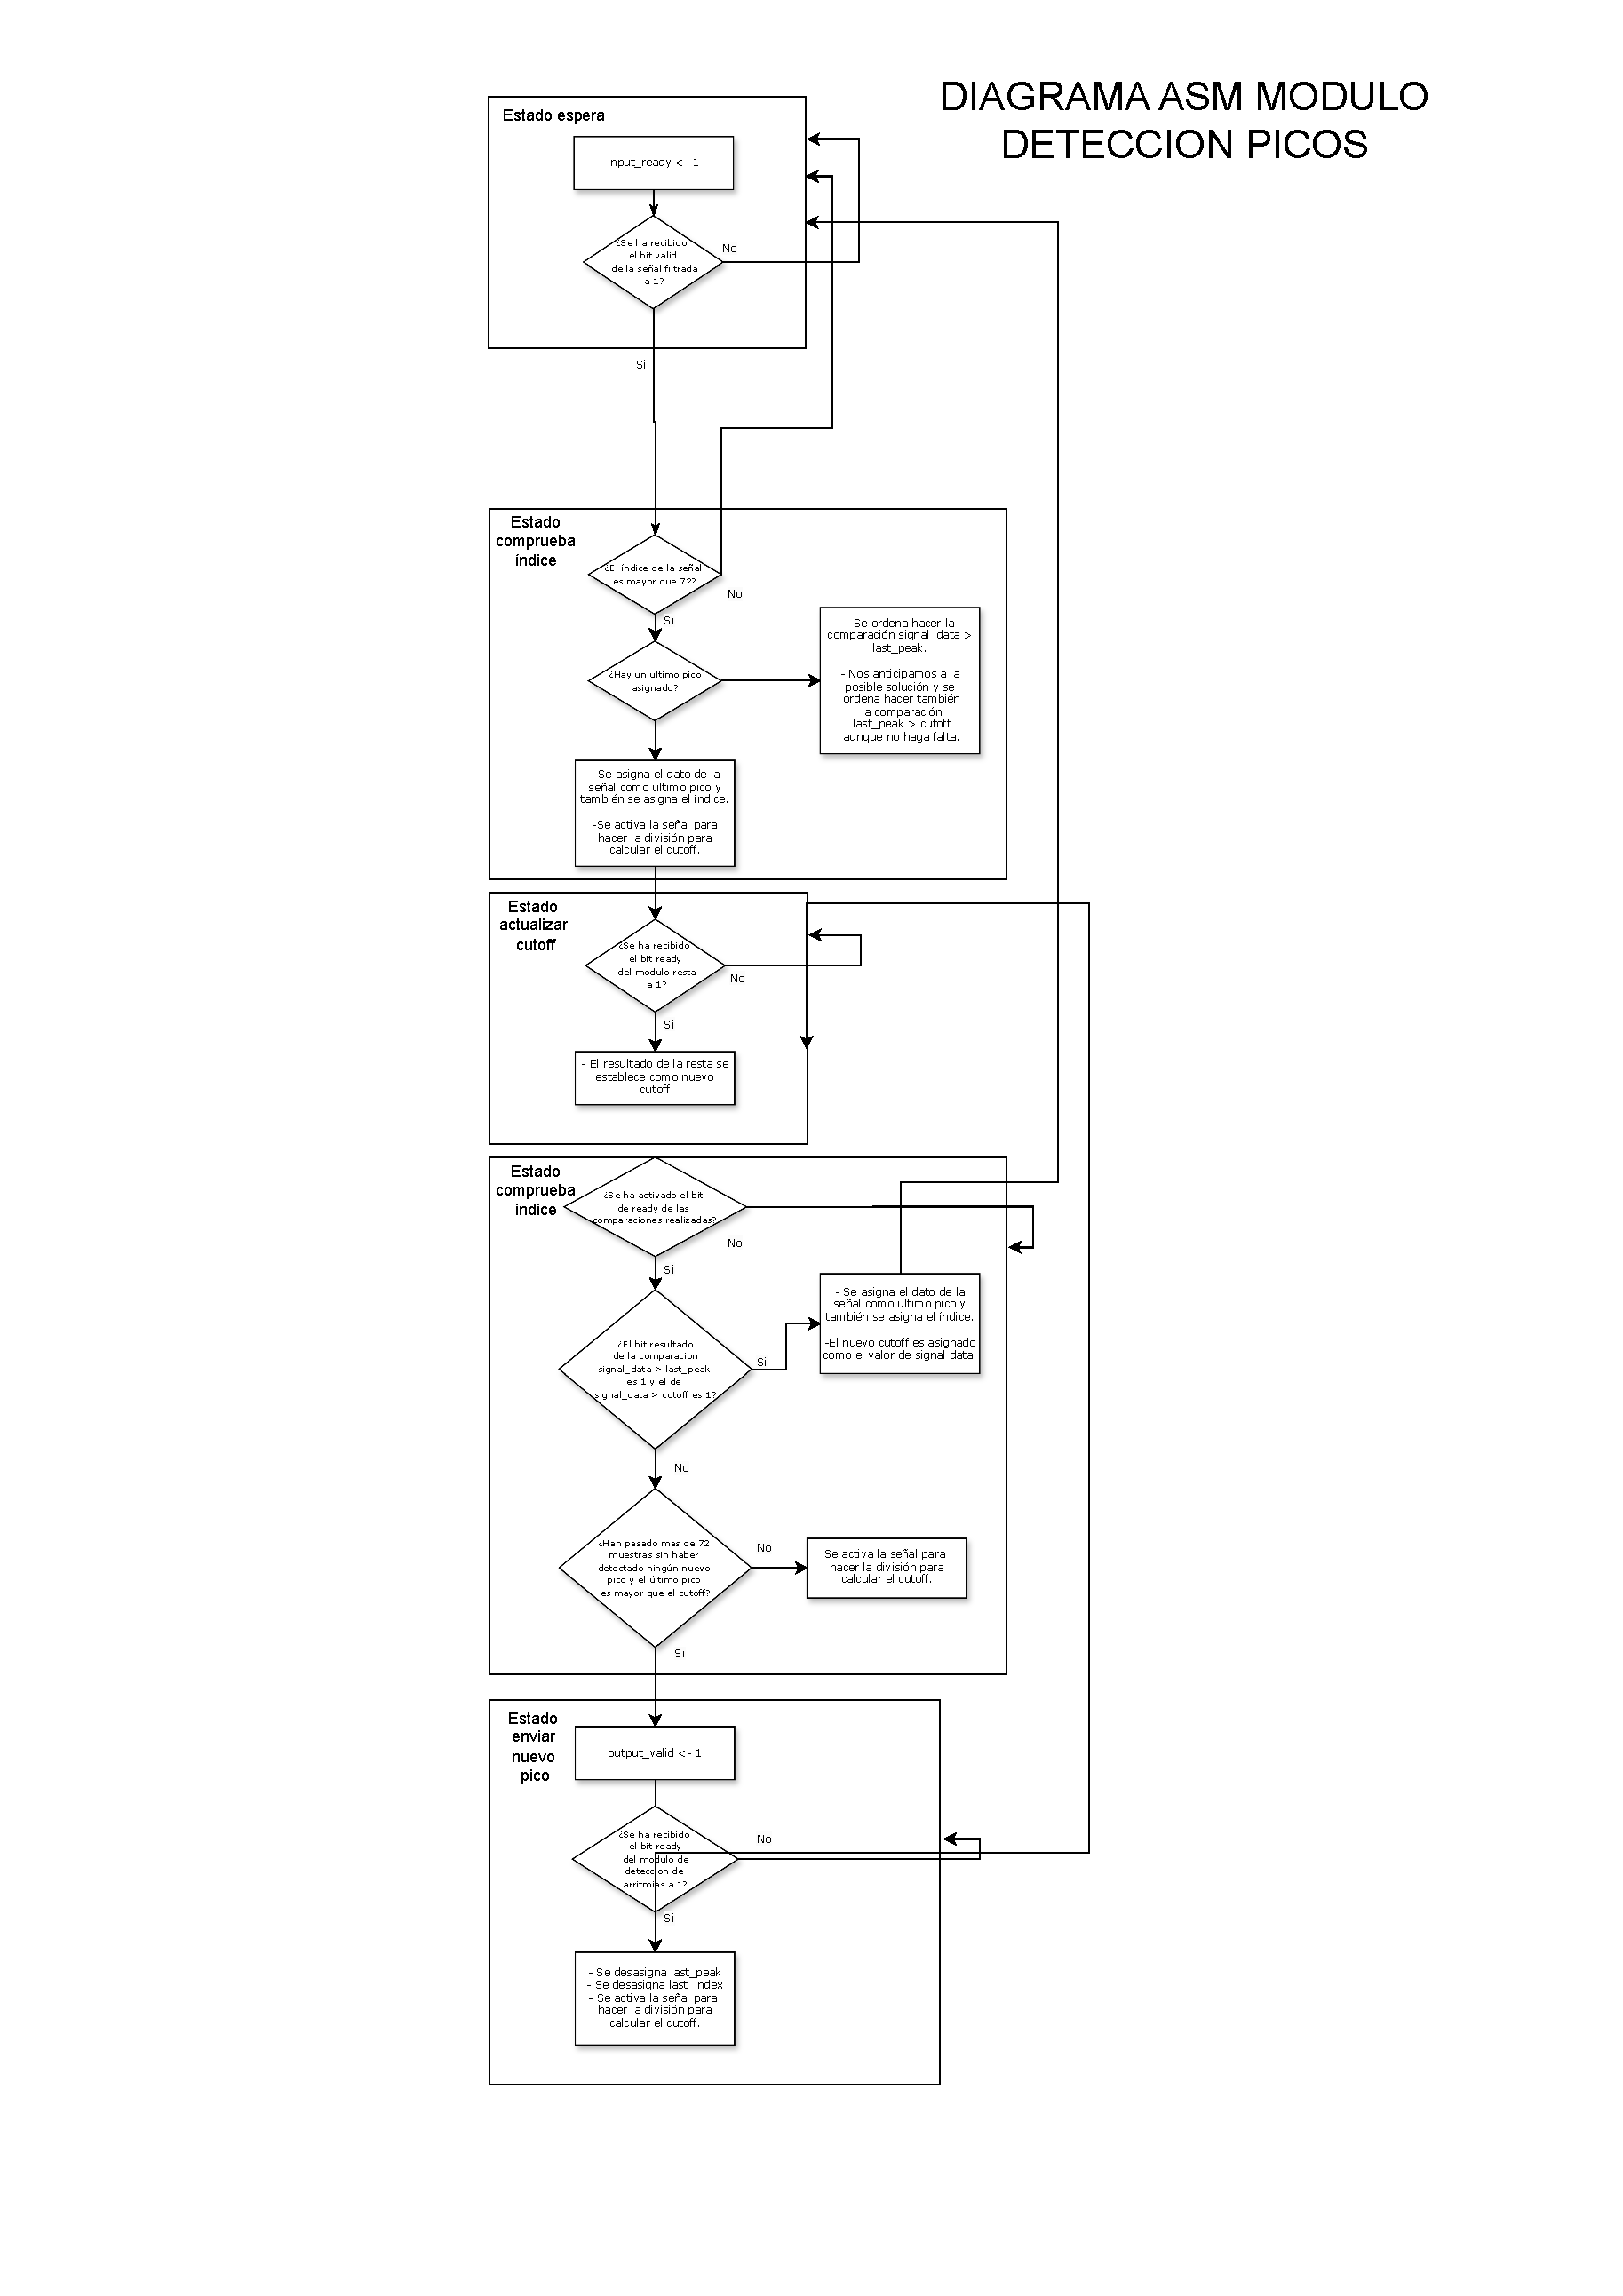
\includegraphics[width=0.99\textwidth]{./Images/img_implementacion_hw/Diagramaasmpicos.pdf}
    \caption{Diagrama asm de Módulo de deteccion de picos}
    \label{fig:Diagramaasmpicos}
\end{figure} 

De manera asincrona se pasa como output el last index pero el módulo de deteccion de arritmias se activa cuando input\_valid
se activa usando asi el last index correspondiente 
\lstset{language=VHDL, breaklines=true, basicstyle=\footnotesize}
\begin{lstlisting}[frame=single]
    output_peak_index <= last_index;
\end{lstlisting}

\section{Módulo de deteccion de arritmias}

El módulo de deteccion de arritmias se encarga de detectar si la distancia entre 2 picos QRS es considerada una arritmia o no,
 
\subsection{Señales de entrada y salida}
las señales de entrada de este módulo son:

\begin{itemize}
    \item clk y reset
    \item input\_peak\_index: señal que recibe las muestras de los picos QRS.
    \item input\_valid e input\_ready: son flags que sirven para sincronizar este módulo con el módulo de deteccion de picos. 
\end{itemize}
    
Las señales de salida son:

\begin{itemize}
    \item output\_arrythmia\_detected: flag que saca 0 si el ritmo es normal y 1 si se ha detectado una arritmia.
    \item output\_arrythmia\_index: valor que indica en que sample se ha producido la arritmia.
    \item output\_valid y output\_ready: para la sincronizacion con el módulo output.
\end{itemize}

\lstset{language=VHDL, breaklines=true, basicstyle=\footnotesize}
\begin{lstlisting}[frame=single]
    Port (
        clk: in std_logic;
        rst: in std_logic;
        
        input_peak_index: in std_logic_vector(31 downto 0); 
        input_valid: in std_logic;
        input_ready: out std_logic;
        
        output_arrythmia_detected: out std_logic; -- ya que saca 0 si es ritmo normal y 1 si es arritmia
        output_arrythmia_index: out std_logic_vector(31 downto 0);
        output_valid: out std_logic;
        output_ready: in std_logic
       );
\end{lstlisting}

\begin{figure}[h!]
    \centering
    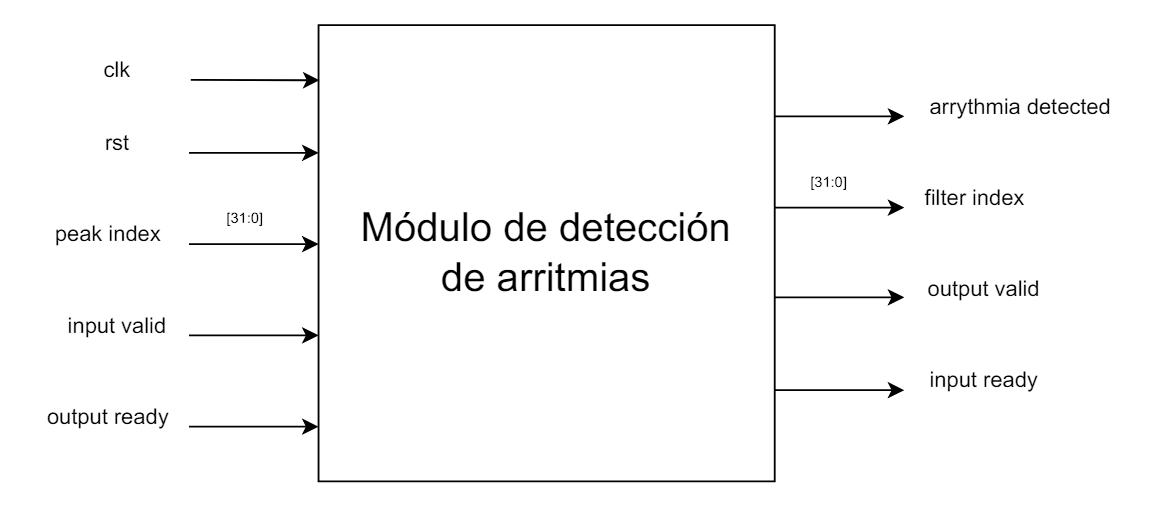
\includegraphics[width=0.6\textwidth]{./Images/img_implementacion_hw/moddeteccionarritmias.png}
    \caption{Entradas y salidas del módulo de deteccion de arritmias}
    \label{fig:moddeteccionarritmias}
\end{figure} 

\subsection{Maquina de estados}

\begin{itemize}
    \item Estado de espera: En el estado de espera se activa la señal de ready y se espera a que se envie un pico QRS, despues pasa al estado S0
    \item Estado S0: Si el contador es 0 significa que se recibe el primer pico registrado por lo que se guarda para mas tarde y se pasa al estado de espera.
    Si el contador es 1 significa que se recibe el segundo pico y por tanto se compara con el anterior hallando la primera distancia despues pasa al estado S1.
    Si no se cumple ninguna condición se pasa al estado S1.    
    \item Estado S1: aumenta el contador en 1, y se calcula la distancia actual.
    \item Estado S2: se actualizan las variables que crean un buffer ficticio y los valores se mueven una posicion cuando se añade la distancia actual como si fuese una cola.
    \item Estado S3: Como ya se explico en la parte de la implementacion del algoritmo TNRange es una señal que simbiliza la distancia entre el pico detectado como arritmia y 
    el pico normal actual, este flag se activa cuando ha habido una arritmia ya que last\_distance puede ser mas grande de lo normal, es por eso que para calcular el gap cuando este flag esta activo
     y el de arritmia detectada no, se compara la distancia actual con la ultima distancia sino con una 3 veces anterior a la última. Si esta condicion no se cumple, para calcular el gap se compara 
     con la ultima distancia, ademas si justo la anterior distancia era la de una arritmia, se desactiva el flag de arritmia detectada.
    \item Estado S4: Se calcula el procentaje de forma asincrona, si el flag de porcentaje es igual a 1 significa que el porcentaje calculado es mayor de lo esperado y por tanto se activan las flags
    de TNRange y counter\_arrythmias. Independientemente despues el indice y la distancia actual pasan a ser last\_distance y last\_index
    \item Estado S5: Se activa la señal de valid y se espera a la señal de ready para que se envie el dato al módulo de output.
\end{itemize}

Se calcula el porcentaje del gap entre las 2 distancias con una distancia normal de forma asincrona.

\begin{itemize}
    \item Estas señales estan en complemento A2 por ello al salir numeros negativos, el bit mas significativo se cambia a 1, es por ello que como solo se consideran los numeros positivos, se
     considera solamente los numeros cuyo bit mas significativo sea 0
    \item como al principio la señal de la ultima distancia es x"00000000" al comparar esta distancia con la actual saldra una distancia enorme que activara el bit del porcentaje que se calcula 
    de forma asincrona asiq ue quitramos ese caso especifico de por medio.
    \item en vez de hacer una division del gap entre distance\_for\_calc se sigue esta fórmula:
    \[ gap/distanceforcalc > 0.15\] 
    \[gap > 0.15 \cdot distanceforcalc \] 
    \[gap > distanceforcalc>> 5 + distanceforcalc>> 3 + distanceforcalc\] 
\end{itemize}

\lstset{language=VHDL, breaklines=true, basicstyle=\footnotesize}
\begin{lstlisting}[frame=single]
    percentage <= '1' when gap(31) = '0' and last_distance > x"00000000" and (std_logic_vector(shift_right(unsigned(distance_for_calc), 3) + shift_right(unsigned(distance_for_calc), 5)) <= std_logic_vector(unsigned(gap))) else '0';
\end{lstlisting}


\begin{figure}[h!]
    \centering
    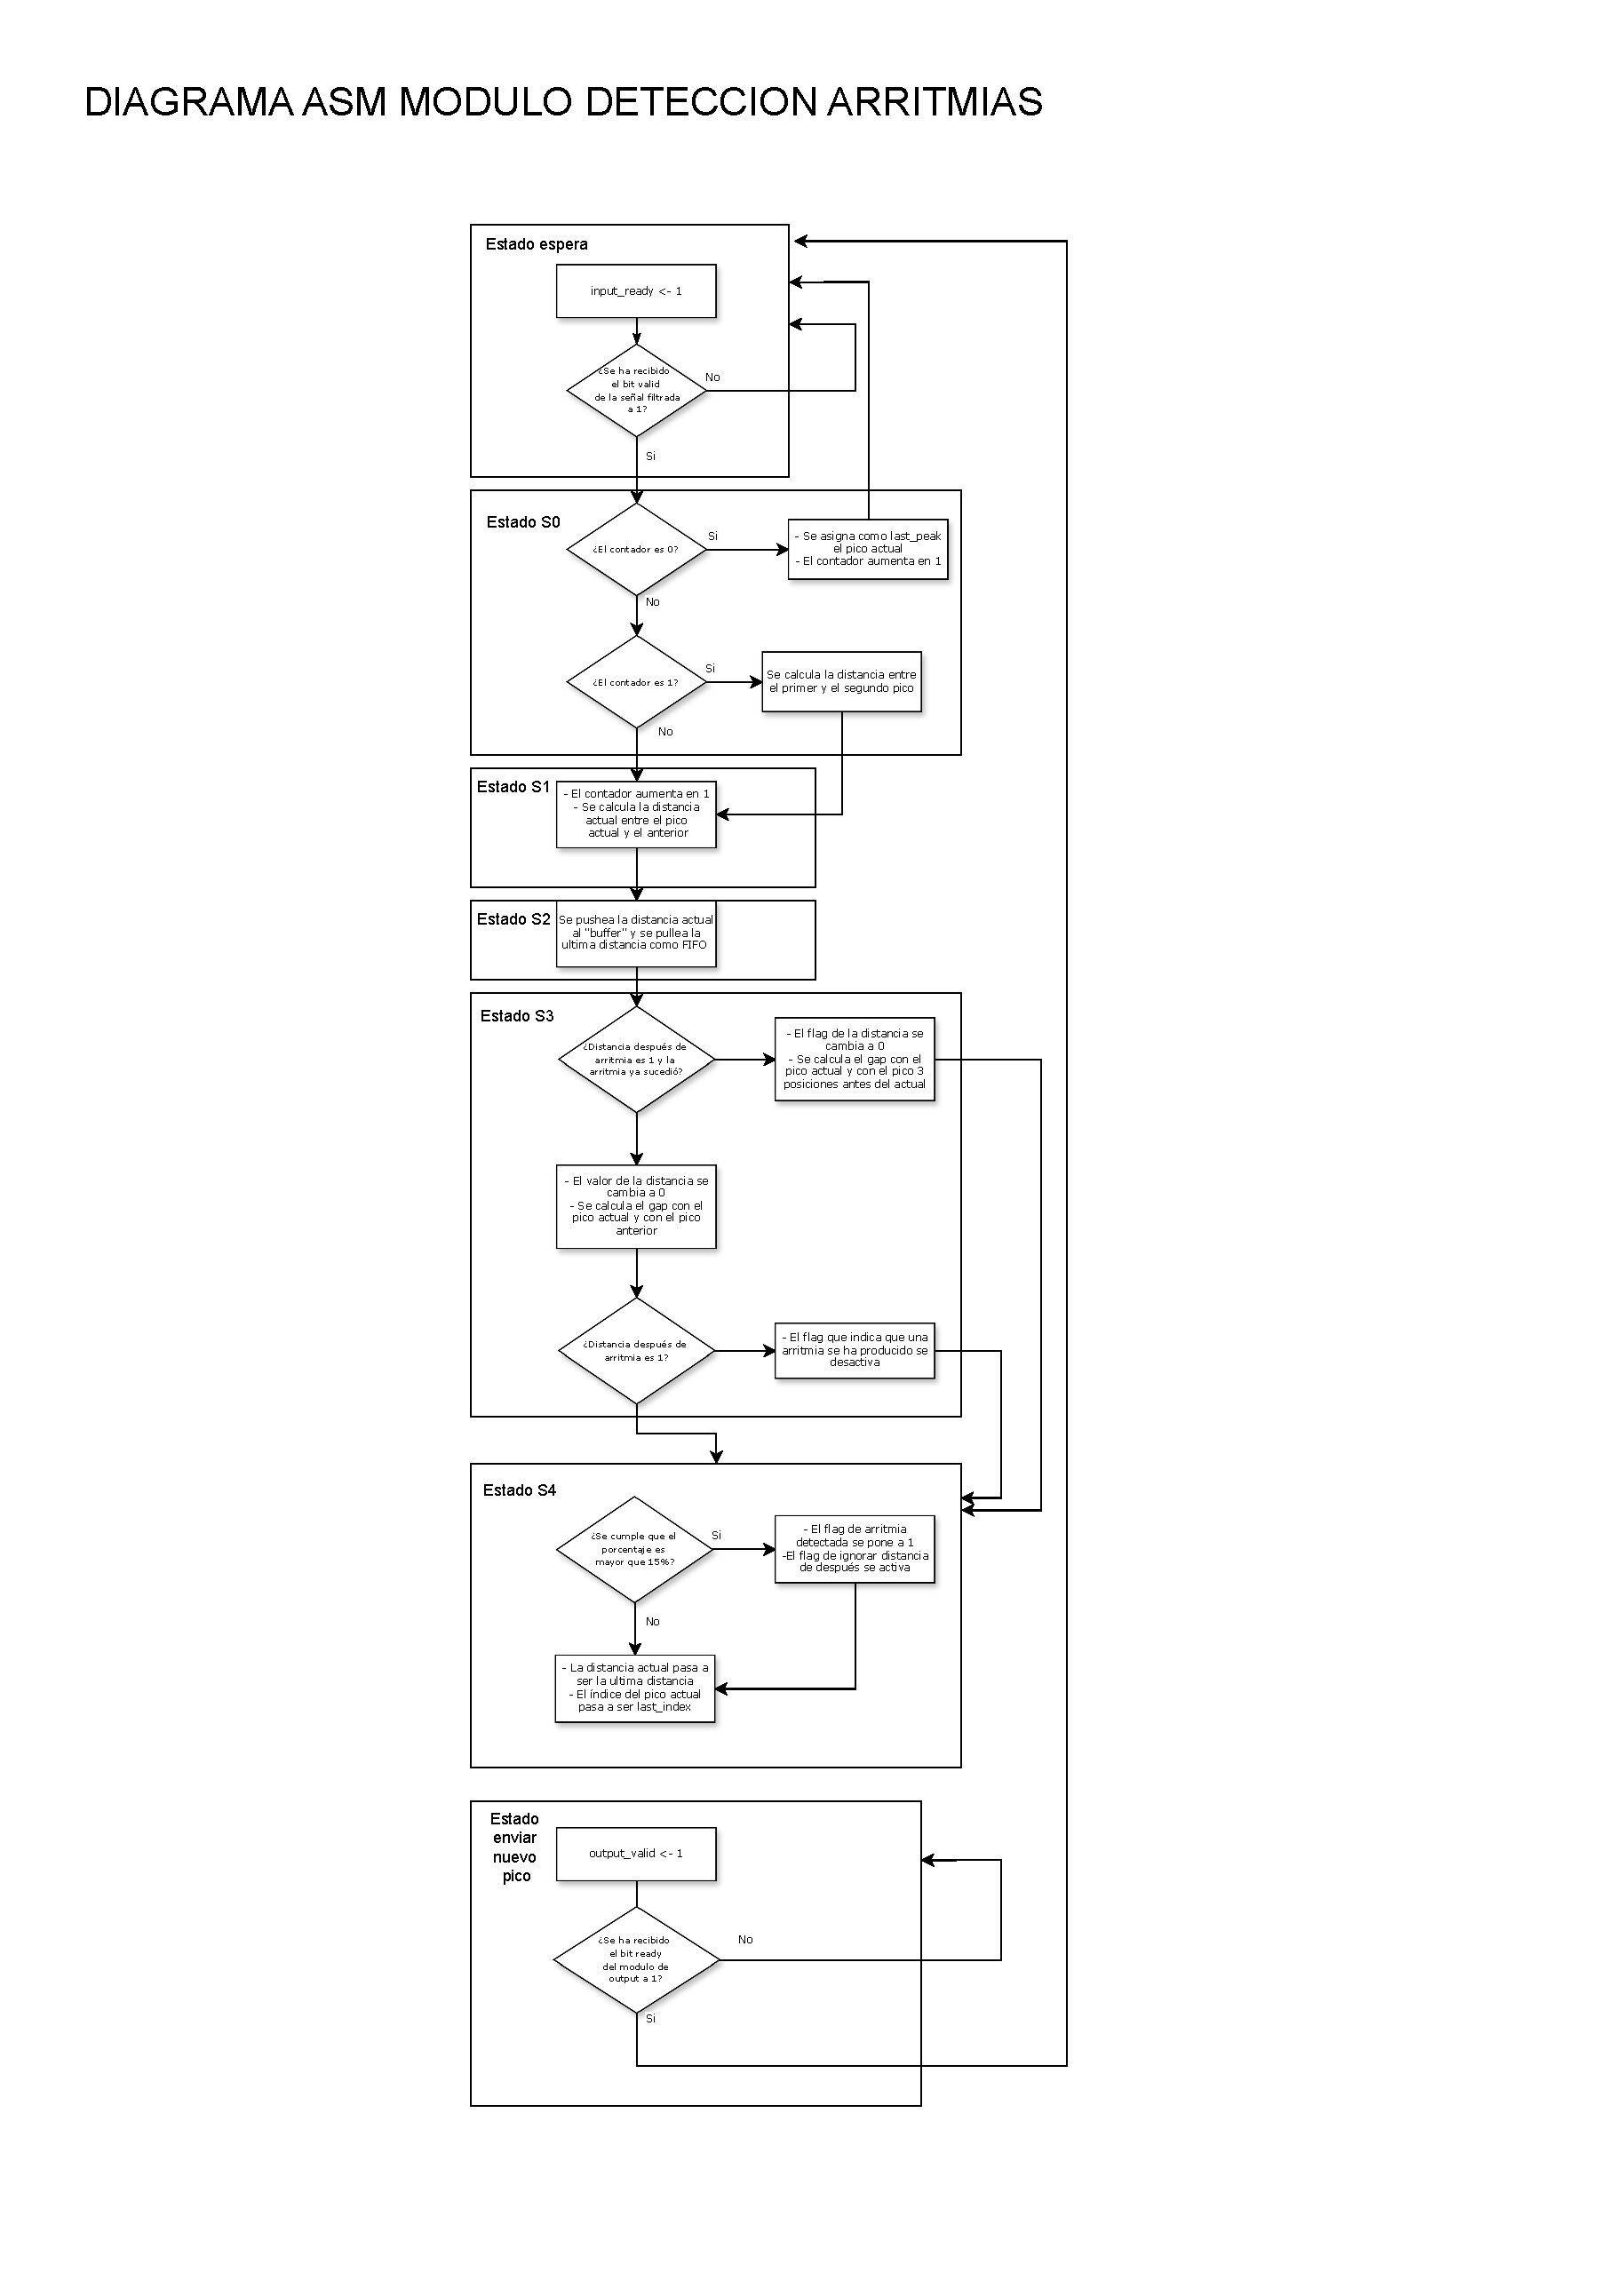
\includegraphics[width=0.99\textwidth]{./Images/img_implementacion_hw/Diagramaasmarritmias.pdf}
    \caption{Diagrama asm de Módulo de filtrado de señal}
    \label{fig:Diagramaasmarritmias}
\end{figure} 

\section {Módulos input y output}
Estos módulos se componen de un estado de lectura y uno de escritura donde uno lee el dato y el otro se encarga de esperar a que se lea el dato y actualizar 
el contador para que se pueda leer de la siguiente posicion de la ROM

\subsection{Módulo input}
\begin{itemize}
    \item Estado de lectura: Primero se asegura de que el contador no hay llegado a la cantidad de muestras máximas en este caso 40625, después pone el bit de enable a 1 
    y pasa al estado de espera.
    \item Estado de espera: pone el bit de valid a 1 y espera al bit de ready para que el siguiente módulo lea el dato, actualiza el contador y pasa al estado de lectura.
\end{itemize}

Este módulo cuenta con una ROM con los valores de la señal original, valores que se van leyendo cundo la señal de ready se activa.

\subsection{Módulo output}
\begin{itemize}
    \item Estado de lectura: Primero se asegura de que el contador no hay llegado a la cantidad de muestras máximas en este caso 144, después pone el bit de enable a 1 
    y pasa al estado de espera. Si se han leido todas las muestras pasa al estado correcto.
    \item Estado de espera: pone el bit de valid a 1 y espera al bit de ready para que el siguiente módulo lea el dato, actualiza el contador y se comprueba si la anotacion
    del pico coincide con la anotacion de la BRAM que es la anotacion original. Ademas se asegura que la anotacion pertenece al indice correcto, si esta condicion se cumple
    sigue con la ejecucion, si no pasa al estado de error.
    \item Estado error: pone la señal de error a 1 y se para la ejecucion ya que un resultado no coincide.
    \item Estado correcto: pone la señal de correcto a 0 que indica que el programa ha sido replicado con exito.
\end{itemize}

Este módulo cuenta con una ROM con las anotaciones de los cardiologos de casa pico QRS, valores que se van leyendo cundo la señal de valid se activa.

\section{Módulo principal y testbench}

El módulo principal se encarga de sincronizar los módulos pasando los datos de un módulo al siguiente asi como la señal de valid y transferir de vuelta la señal de ready.

Tambien se ha definido un testbench donde se definen los ciclos de reloj, ademas del reset al principio de la ejecucion. Como salida tiene los estados correcto y error para 
ver los resultados de la ejecucion.

\section{Otros módulos} 
explicar módulos de punto flotante y ROM/RAM pero mover
arriba para que sean los primeros módulos que se expliquen
\subsection{Módulos ROM y RAM}
 ROM muestras

\begin{figure}[h!]
    \centering
    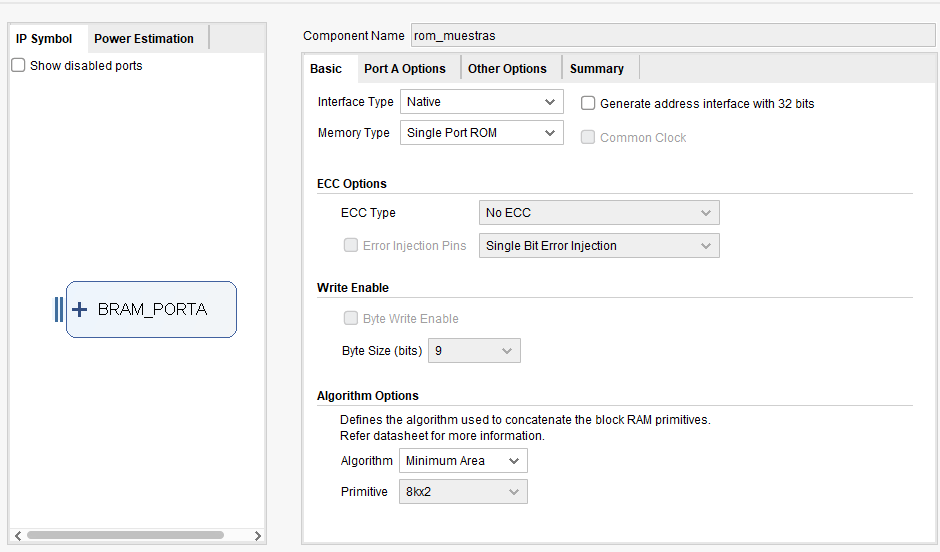
\includegraphics[width=0.6\textwidth]{./Images/img_implementacion_hw/rom_muestras_1.png}
    \caption{Seleccion de la opcion simple block ROM y}
    \label{fig:rom_muestras_1}
\end{figure}
 Es importante desactivar l a opcion de primitive output para que no se añada un registro extra 
 al principio y la simulacion se ejecute en cada tiempo correspondiente. 
\begin{figure}[h!]
    \centering
    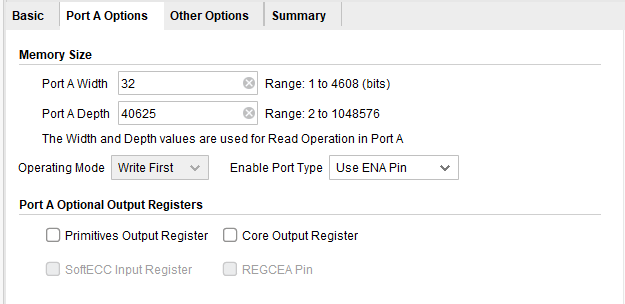
\includegraphics[width=0.6\textwidth]{./Images/img_implementacion_hw/rom_muestras_2.png}
    \caption{Se establecen las filas de la BROM y la longitud de estas}
    \label{fig:rom_muestras_2}
\end{figure}

El módulo de filtrado utiliza 1 ROM y una RAM

\begin{itemize}
\item La ROM se configura igual que la ROM del módulo de input, este tiene 99 filas y de anchura 
tiene 32 bits.
\item La RAM se configura como single port RAM y se mantiene desactivado el valor de primitive output.
 Ahora bien los valores asignados son los siguientes.
 
\begin{figure}[h!]
    \centering
    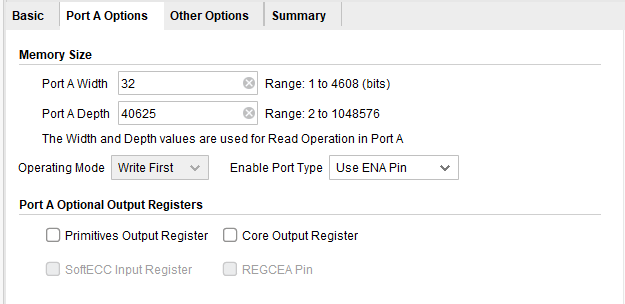
\includegraphics[width=0.6\textwidth]{./Images/img_implementacion_hw/rom_muestras_2.png}
    \caption{Se establecen las filas de lectura y escritura de la RAM y las longitud de dichas filas}
    \label{fig:ram_muestras_1}
\end{figure}

\end{itemize}

\subsection{Módulos punto flotante}

Se han definido varios módulos para hacer las distintas operaciones en punto flotante ya que en VHDL no se
pueden hacer estas operaciones directamente, se necesitan usar otros módulos especializados para estas operaciones.

Como se operan con valores en punto flotante simple, las señales tienen que ser de 32 bits y por simplificar el
codigo, casi todos los valores tanto en punto flotante como enteros se declaran con señales de 32 bits.

En este programa se necesitan 5 tipos de módulos de operaciones.

\begin{itemize}
    \item Módulo comparador mayor que: se utiliza para comparar varias señales en el módulo de deteccion de picos como son:
    \begin{itemize}
        \item signal\_data gt last\_peak
        \item signal\_data gt cutoff
        \item last\_peak gt cutoff
    \end{itemize}

    \begin{figure}[h!]
        \centering
        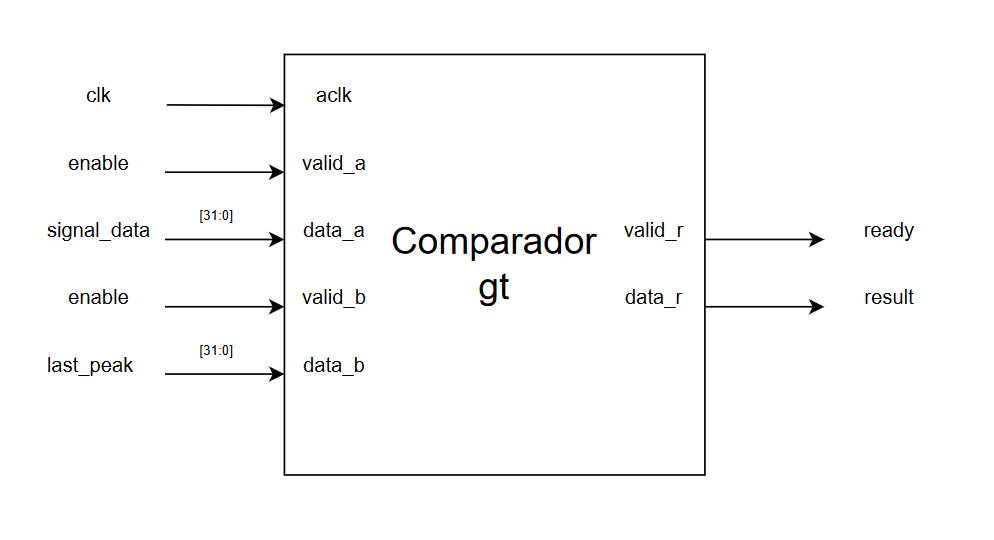
\includegraphics[width=0.8\textwidth]{./Images/img_implementacion_hw/comparadorgt.png}
        \caption{Entrada y salida del módulo de comparador}
        \label{fig:comparadorgt}
    \end{figure}

    \item Módulo divisor y resta: se utilizan en conjunto para calcular el cutoff que tiene la operacion:
    \[cutoff = cutoff - cutoff/192\]
    \begin{figure}[h!]
        \centering
        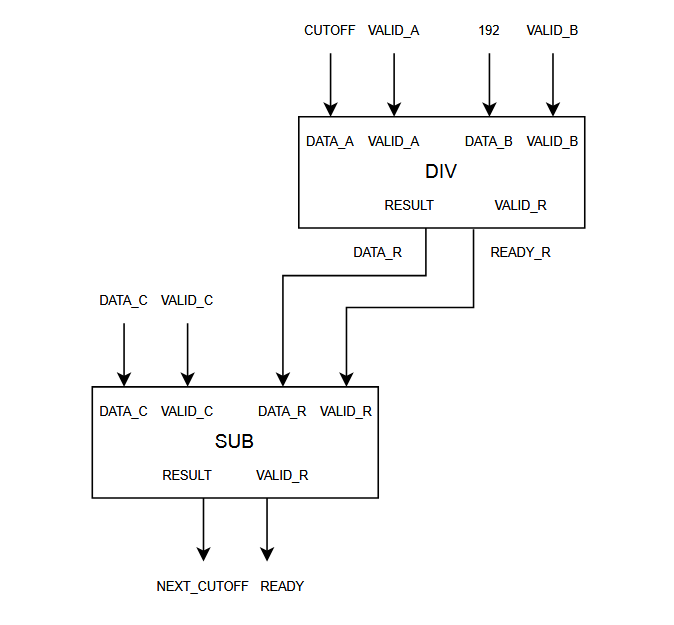
\includegraphics[width=0.9\textwidth]{./Images/img_implementacion_hw/DiagramaDivisorrestador.png}
        \caption{Funcionamiento de la conexion de los módulos de divisor y restador}
        \label{fig:divisorrestador}
    \end{figure}   
    \item Modulo multiplicacion: Se usa para poder multiplicar los valores de las muestras con los valores de los coeficientes en el modulo de filtrado.
\end{itemize}
